% lintrans - The linear transformation visualizer
% Copyright (C) 2021-2022 D. Dyson (DoctorDalek1963)

% This program is licensed under GNU GPLv3, available here:
% <https://www.gnu.org/licenses/gpl-3.0.html>

\documentclass[../development.tex]{subfiles}

\begin{document}

\subsubsection{Asking strangers on the internet for help\label{development:visualizing-matrices:asking-strangers-on-the-internet-for-help}}

After creating most of the GUI skeleton, I wanted to build the viewport. Unfortunately, I had no idea what I was doing.

While looking through the PyQt5 docs, I found a pretty comprehensive explanation of the Qt5 \enquote{Graphics View Framework}\cite{pyqt5-graphics-view-framework}, which seemed pretty good, but not really what I was looking for. I wanted a way to easily draw lots of straight, parallel lines. This framework seemed more focussed on manipulating objects on a canvas, almost like sprites. I knew of a different Python library called \texttt{matplotlib}, which has various backends available. I learned that it could be embedded in a standard PyQt5 GUI, so I started doing some research.

I didn't get very far with \texttt{matplotlib}. I hadn't used it much before and it's designed for visualizing data. It can draw manually defined straight lines on a canvas, but that's not what it's designed for and it's not very good at it. Thankfully, my horrific \texttt{matplotlib} code has been lost to time. I used the \texttt{Qt5Agg} backend from \texttt{matplotlib} to create a custom PyQt5 widget for the GUI and I could graph randomly generated data with it after following a tutorial\cite{matplotlib-pyqt5-tutorial}.

I realised that I wasn't going to get very far with \texttt{matplotlib}, but I didn't know what else to do. I couldn't find any relevant examples on the internet, so I decided to post a question on a forum myself. I'd had experience with StackOverflow and its unfriendly community before, so I decided to ask the \texttt{r/learnpython} subreddit\cite{reddit-framework-question}.

I only got one response, but it was incredibly helpful. The person told me that if I couldn't find an easy way to do what I wanted, I could write a custom PyQt5 widget. I knew this was possible with a class that just inherited from \texttt{QWidget}, but had no idea how to actually make something useful. Thankfully, this person provided a link to a GitLab repository of theirs, where they had multiple examples of custom widgets with PyQt5\cite{gitlab-custom-widgets}.

When looking through this repo, I found out how to draw on a widget like a simple canvas. All I have to do is override the \texttt{paintEvent()} method and use a \texttt{QPainter} object to draw on the widget. I used this knowledge to start creating the actual viewport for the GUI, starting with the background axes.

\subsubsection{Creating the plots package\label{development:visualizing-matrices:creating-the-plots-package}}

Initially, the \texttt{lintrans.gui.plots} package just has some classes for widgets. \texttt{TransformationPlotWidget} acts as a base class and then \texttt{ViewTransformationWidget} acts as a wrapper. I will expand this class in the future.

%: 4af63072b383dc9cef9adbb8900323aa007e7f26
%: src/lintrans/gui/plots/plot_widget.py

\fsbsl{development/4af63072b383dc9cef9adbb8900323aa007e7f26/gui.png}{The GUI with background axes}{The meat of this class is the \texttt{draw_widget()} method. Right now, this method only draws the background axes. My next step is to implement basis vector attributes and draw them in \texttt{draw_widget()}. After changing the the \texttt{plot} attribute in \texttt{LintransMainWindow} to an instance of \texttt{ViewTransformationWidget}, the plot was visible in the GUI.\par I then refactored the code slightly to rename \texttt{draw_widget()} to \texttt{draw_background()} and then call it from the \texttt{paintEvent()} method in \texttt{ViewTransformationWidget}.}

\subsubsection{Implementing basis vectors\label{development:visualizing-matrices:implementing-basis-vectors}}

My first step in implementing basis vectors was to add some utility methods to convert between coordinate systems. The matrices are using Cartesian coordinates with $(0, 0)$ in the middle, positive $x$ going to the right, and positive $y$ going up. However, Qt5 is using standard computer graphics coordinates, with $(0, 0)$ in the top left, positive $x$ going to the right, and positive $y$ going down. I needed a way to convert Cartesian \enquote{grid} coordinates to Qt5 \enquote{canvas} coordinates, so I wrote some little utility methods.

%: 1fa7e1c61d61cb6aeff773b9698541f82fee39ea
%: src/lintrans/gui/plots/plot_widget.py:45-60

Once I had a way to convert coordinates, I could add the basis vectors themselves. I did this by creating attributes for the points in the constructor and creating a \texttt{transform_by_matrix()} method to change these point attributes accordingly.

%: 37e7c208a33d7cbbc8e0bb6c94cd889e2918c605
%: src/lintrans/gui/plots/plot_widget.py:92-112

I also created a \texttt{draw_transformed_grid()} method which gets called in \texttt{paintEvent()}.

%: 37e7c208a33d7cbbc8e0bb6c94cd889e2918c605
%: src/lintrans/gui/plots/plot_widget.py:122-128

I then changed the \texttt{render_expression()} method in \texttt{LintransMainWindow} to call this new \texttt{transform_by_matrix()} method.

%: 37e7c208a33d7cbbc8e0bb6c94cd889e2918c605
%: src/lintrans/gui/main_window.py:229-235

Testing this new code shows that it works well.

\begin{figure}[H]
	\centering
	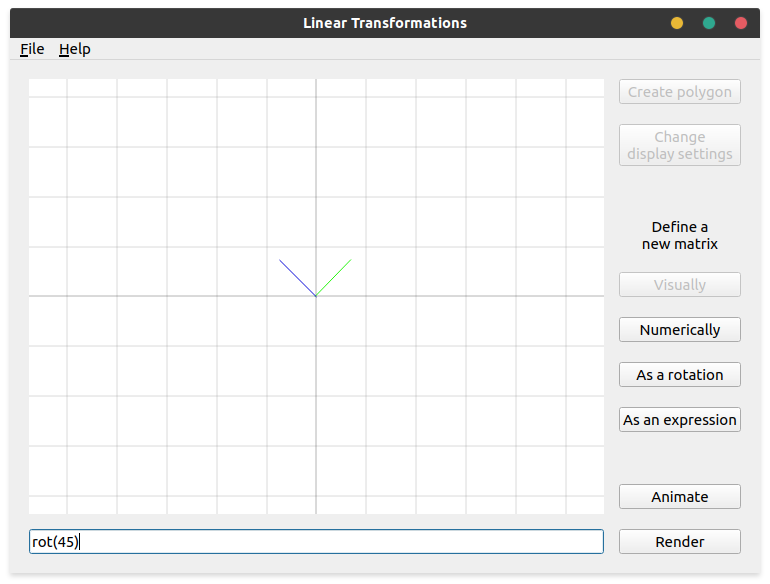
\includegraphics[width=0.7\linewidth]{development/37e7c208a33d7cbbc8e0bb6c94cd889e2918c605/gui.png}
	\caption{Basis vectors drawn for a $45\degree$ rotation}
	\label{fig:development:37e7c208a33d7cbbc8e0bb6c94cd889e2918c605:gui.png}
\end{figure}

\subsubsection{Drawing the transformed grid\label{development:visualizing-matrices:drawing-the-transformed-grid}}

After drawing the basis vectors, I wanted to draw the transformed version of the grid. I first created a \texttt{grid_corner()} utility method to return the grid coordinates of the top right corner of the canvas. This allows me to find the bounding box in which to draw the grid lines.

%: 2ade98ac28d1c3f6691e4afa819142a3ab8e9fd9
%: src/lintrans/gui/plots/plot_widget.py:64-66

I then created a \texttt{draw_parallel_lines()} method that would fill the bounding box with a set of lines parallel to a given vector with spacing defined by the intersection with a given point.

%: 2ade98ac28d1c3f6691e4afa819142a3ab8e9fd9
%: src/lintrans/gui/plots/plot_widget.py:126-164

I then called this method from \texttt{draw_transformed_grid()}.

%: 2ade98ac28d1c3f6691e4afa819142a3ab8e9fd9
%: src/lintrans/gui/plots/plot_widget.py:166-178

\fsbsr{development/2ade98ac28d1c3f6691e4afa819142a3ab8e9fd9/gui.png}{Parallel lines being drawn for matrix $1.2\mathbf{I}$}{This worked quite well when the matrix involved no rotation, as seen on the right, but this didn't work with rotation. When trying \pyinline{'rot(45)'} for example, it looked the same as in Figure~\ref{fig:development:37e7c208a33d7cbbc8e0bb6c94cd889e2918c605:gui.png}.\par Also, the vectors aren't particularly clear. They'd be much better with arrowheads on their tips, but this is just a prototype. The arrowheads will come later.\par My next step was to make the transformed grid lines work with rotations.}

%: 7dfe1e24729562501e2fd88a839dca6b653a3375
%: src/lintrans/gui/plots/plot_widget.py:126-225

This code checks if $x$ or $y$ is zero\footnote{We actually check if they're less than $10^{-12}$ to allow for floating point errors} and if they're not, then we have to use the standard straight line equation $y = mx + c$ to create parallel lines. We find our value of $m$ and then iterate through all the values of $c$ that keep the line within the bounding box.

\fsbsl{development/7dfe1e24729562501e2fd88a839dca6b653a3375/gui.png}{An example of a $20\degree$ rotation}{There are some serious logical errors in this code. It works fine for things like \pyinline{'3rot(45)'} or \pyinline{'0.5rot(20)'}, but something like \pyinline{'rot(115)'} will leave the program hanging indefinitely.\par In fact, this code only works for rotations between $0\degree$ and $90\degree$, and will hang forever when given a matrix like $\begin{psmallmatrix}12 & 4 \\ -2 & 3\end{psmallmatrix}$, because it's just not very good.\par I will fix these issues in the future, but it works somewhat decently, so I decided to do animation next, because that sounded more fun.}

\subsubsection{Implementing animation\label{development:visualizing-matrices:implementing-animation}}

Now that I had a very crude renderer, I could create a method to animate a matrix. Eventually I want to be able to apply a given matrix to the currently rendered scene and animate between them. However, I wanted to start simple by animating from the identity to the given matrix.

%: 829a130af5aee9819bf0269c03ecfb20bec1a108
%: src/lintrans/gui/main_window.py:238-258

This code creates the \texttt{matrix_move} variable and adds scaled versions of it to the identity matrix and renders that each frame. It's simple, but it works well for this simple use case. Unfortunately, it's very hard to show off an animation in a PDF, since all these images are static. The git commit hashes are included in the code snippets if you want to clone the repo\cite{lintrans-github}, checkout this commit, and run it yourself if you want.

\subsubsection{Preserving determinants\label{development:visualizing-matrices:preserving-determinants}}

Ignoring the obvious flaw with not being able to render transformations with a more than $90\degree$ rotation, the animations don't respect determinants. When rotating $90\degree$, the determinant changes during the animation, even though we're going from a determinant 1 matrix (the identity) to another determinant 1 matrix. This is because we're just moving each vector to its new position in a straight line. I want to animate in a way that smoothly transitions the determinant.

\begin{figure}[H]
	\hspace{0.005\linewidth}
	\centering
	\begin{minipage}{0.48\linewidth}
		\centering
		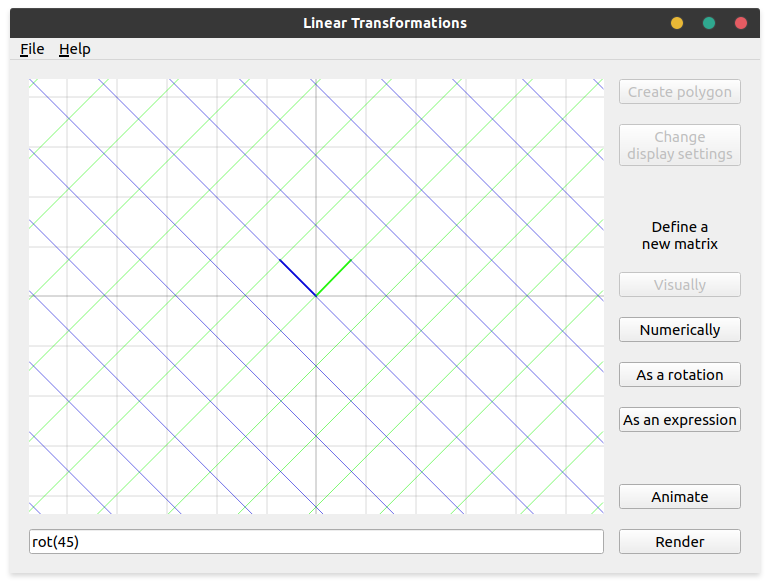
\includegraphics[width=\linewidth]{development/3fa1bdee4a106cb32a55d1364d606f75365f6fd1/gui-expected.png}
		\caption{What we would expect halfway through a $90\degree$ rotation}
		\label{fig:development:3fa1bdee4a106cb32a55d1364d606f75365f6fd1:gui-expected.png}
	\end{minipage}\hspace{0.015\linewidth}
	\begin{minipage}{0.48\linewidth}
		\centering
		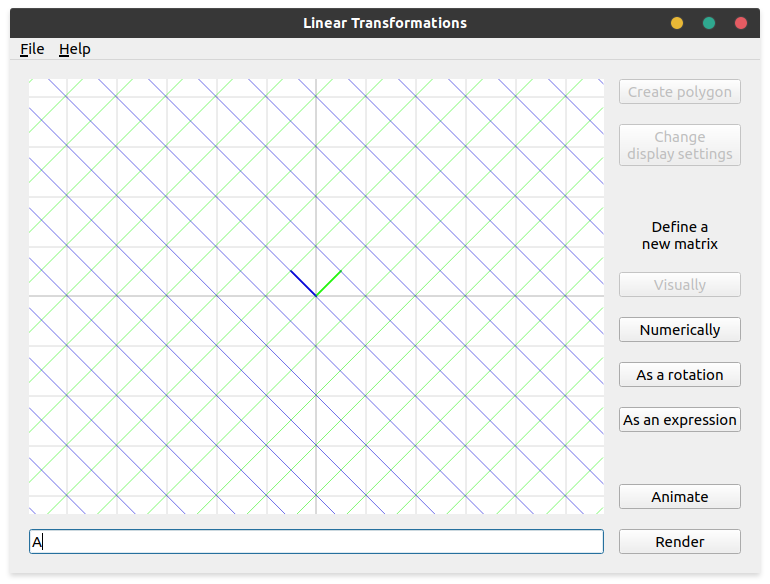
\includegraphics[width=\linewidth]{development/3fa1bdee4a106cb32a55d1364d606f75365f6fd1/gui-reality.png}
		\caption{What we actually get halfway through a $90\degree$ rotation}
		\label{fig:development:3fa1bdee4a106cb32a55d1364d606f75365f6fd1:gui-reality.png}
	\end{minipage}
	\hspace{0.005\linewidth}
	\vspace{-1em}
\end{figure}

In order to smoothly animate the determinant, I had to do some maths. I first defined the matrix $\mathbf{A}$ to be equivalent to the \texttt{matrix_move} variable from before - the target matrix minus the identity, scaled by the proportion. I then wanted to normalize $\mathbf{A}$ so that it had a determinant of 1 so that I could scale it up with the \texttt{proportion} variable through the animation.

I think I first tried just multiplying $\mathbf{A}$ by $\dfrac{1}{\det(\mathbf{A})}$ but that didn't work, so I googled it. I found a post\cite{researchgate-normalize-determinant} on ResearchGate about the topic, and thanks to a very helpful comment from Jeffrey~L~Stuart, I learned that for a $2 \times 2$ matrix $\mathbf{A}$ and a scalar $c$, $\det(c \mathbf{A}) = c^2 \det(\mathbf{A})$.

I wanted a $c$ such that $\det(c \mathbf{A}) = 1$. Therefore $c = \dfrac{1}{\sqrt{|\det(\mathbf{A})|}}$. I then defined matrix $\mathbf{B}$ to be $c\mathbf{A}$.

Then I wanted to scale this normalized matrix $\mathbf{B}$ to have the same determinant as the target matrix $\mathbf{T}$ using some scalar $d$. We know that $\det(d \mathbf{B}) = d^2 \det(\mathbf{B}) = \det(\mathbf{T})$. We can just rearrange to find $d$ and get $d = \sqrt{\left|\dfrac{\det(\mathbf{T})}{\det(\mathbf{B})}\right|}$. But $\mathbf{B}$ is defined so that $\det(\mathbf{B}) = 1$, so we can get $d = \sqrt{|\det(\mathbf{T})|}$.

However, we want to scale this over time with our \texttt{proportion} variable $p$, so our final scalar $s = 1 + p \left(\sqrt{|\det(\mathbf{T})|} - 1\right)$. We define a matrix $\mathbf{C} = s \mathbf{B}$ and render $\mathbf{C}$ each frame. When in code form, this is the following:

%: 6ff49450d8438ea2b2e7d2a97125dc518e648bc5
%: src/lintrans/gui/main_window.py:245-290

Unfortunately, the system I use to render matrices is still quite bad at its job. This makes it hard to test properly. But, transformations like \pyinline{'2rot(90)'} work exactly as expected, which is very good.

\end{document}
